\documentclass[tikz,border=8pt]{standalone}
\usepackage{tikz}
\usetikzlibrary{shapes.geometric,arrows.meta,positioning,fit,backgrounds}

\begin{document}
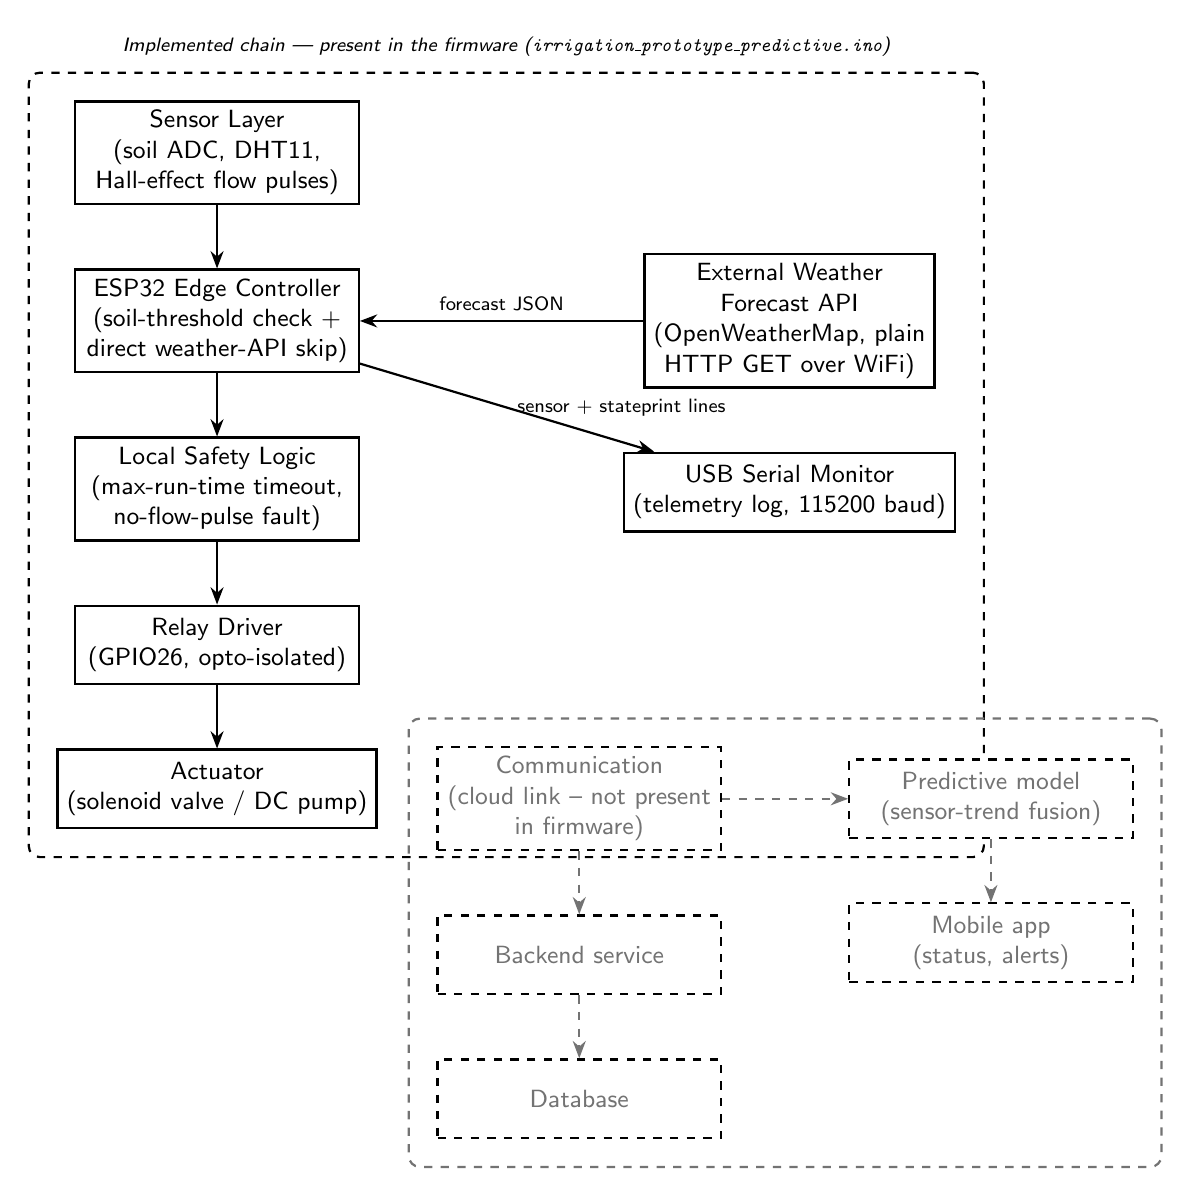
\begin{tikzpicture}[
  font=\sffamily\small,
  box/.style={draw, thick, rectangle, minimum width=3.6cm, minimum height=1cm, align=center, fill=white},
  propbox/.style={draw, thick, dashed, rectangle, minimum width=3.6cm, minimum height=1cm, align=center, fill=white, text=black!55},
  arr/.style={-{Stealth[length=2.2mm]}, thick},
  proparr/.style={-{Stealth[length=2.2mm]}, thick, dashed, draw=black!55},
  dashedbox/.style={draw, thick, dashed, inner sep=10pt, rounded corners}
]

% =====================================================================
% IMPLEMENTED CHAIN -- matches irrigation_prototype_predictive.ino
% =====================================================================
\node[box] (sensors) {Sensor Layer\\(soil ADC, DHT11,\\Hall-effect flow pulses)};
\node[box, below=0.8cm of sensors] (esp32) {ESP32 Edge Controller\\(soil-threshold check +\\direct weather-API skip)};
\node[box, below=0.8cm of esp32] (safety) {Local Safety Logic\\(max-run-time timeout,\\no-flow-pulse fault)};
\node[box, below=0.8cm of safety] (driver) {Relay Driver\\(GPIO26, opto-isolated)};
\node[box, below=0.8cm of driver] (actuator) {Actuator\\(solenoid valve / DC pump)};

\draw[arr] (sensors) -- (esp32);
\draw[arr] (esp32) -- (safety);
\draw[arr] (safety) -- (driver);
\draw[arr] (driver) -- (actuator);

\node[box, right=3.6cm of esp32] (weather) {External Weather\\Forecast API\\(OpenWeatherMap, plain\\HTTP GET over WiFi)};
\draw[arr] (weather) -- (esp32) node[midway, above, font=\sffamily\scriptsize] {forecast JSON};

\node[box, below=0.8cm of weather] (serial) {USB Serial Monitor\\(telemetry log, 115200 baud)};
\draw[arr] (esp32) -- (serial) node[midway, right, font=\sffamily\scriptsize] {sensor + state\\print lines};

% =====================================================================
% PROPOSED / NOT-YET-IMPLEMENTED EXTENSION
% =====================================================================
\node[propbox, below=2.6cm of safety, xshift=4.6cm] (comm) {Communication\\(cloud link -- not present\\in firmware)};
\node[propbox, below=0.8cm of comm] (backend) {Backend service};
\node[propbox, below=0.8cm of backend] (db) {Database};
\node[propbox, right=1.6cm of comm] (predictor) {Predictive model\\(sensor-trend fusion)};
\node[propbox, below=0.8cm of predictor] (app) {Mobile app\\(status, alerts)};

\draw[proparr] (comm) -- (backend);
\draw[proparr] (backend) -- (db);
\draw[proparr] (comm) -- (predictor);
\draw[proparr] (predictor) -- (app);

\begin{scope}[on background layer]
\node[dashedbox, fit=(sensors)(actuator)(weather)(serial)] (localbox) {};
\node[font=\sffamily\scriptsize\itshape, align=left, above=2pt of localbox.north, anchor=south]
  {Implemented chain --- present in the firmware (\texttt{irrigation\_prototype\_predictive.ino})};
\node[dashedbox, draw=black!55, fit=(comm)(backend)(db)(predictor)(app)] (remotebox) {};
\end{scope}

\end{tikzpicture}
\end{document}
